\documentclass[../index.tex]{subfiles}

\begin{document}
    % 2.1
    \section{Giới thiệu về C\#}
    \begin{figure}[H]
        \centering
        
\includegraphics[width=0.6\linewidth]{figures/tech-logo/csharp-dotnet.png}
        \caption{C\# \& .NET Core}
    \end{figure}
    \begin{itemize}
        \item \textbf{Khái niệm}: C\# là một ngôn ngữ lập trình hướng đối tượng,
            mạnh mẽ và hiện đại, được phát triển bởi Microsoft.

        \item \textbf{Ưu điểm}:
            \begin{itemize}
                \item Đa nền tảng: Có thể chạy trên nhiều hệ điều hành nhờ .NET Core.

                \item Dễ học: Cú pháp rõ ràng, gần gũi với ngôn ngữ tự nhiên.

                \item Cộng đồng lớn: Có nhiều tài liệu, thư viện và hỗ trợ từ cộng
                    đồng.

                \item Hỗ trợ phát triển ứng dụng đa dạng: desktop, web và mobile.
            \end{itemize}

        \item \textbf{Ứng dụng trong dự án}: C\# .NET 8 được sử dụng để phát triển
            phần backend của ứng dụng, xử lý logic nghiệp vụ và tương tác với cơ
            sở dữ liệu.
    \end{itemize}

    % 2.2
    \section{PostgreSQL}
    \begin{figure}[H]
        \centering
        
\includegraphics[width=0.2\linewidth]{figures/tech-logo/postgres.png}
        \caption{PostgreSQL}
    \end{figure}
    \begin{itemize}
        \item \textbf{Khái niệm}: PostgreSQL là một hệ quản trị cơ sở dữ liệu quan
            hệ mã nguồn mở, mạnh mẽ và đáng tin cậy.

        \item \textbf{Ưu điểm}:
            \begin{itemize}
                \item Mở rộng: Hỗ trợ nhiều loại kiểu dữ liệu, ACID, và các tính
                    năng nâng cao khác.

                \item Hiệu năng cao: Tối ưu hóa cho các truy vấn phức tạp và xử
                    lý dữ liệu lớn.

                \item Cộng đồng lớn: Có nhiều tài liệu, công cụ và hỗ trợ từ cộng
                    đồng.
            \end{itemize}

        \item \textbf{Ứng dụng trong dự án}: PostgreSQL sẽ được sử dụng làm cơ sở
            dữ liệu chính để lưu trữ thông tin người dùng, bài viết, bình luận,
            và các dữ liệu khác của diễn đàn.
    \end{itemize}

    % 2.3
    \section{Redis}
    \begin{figure}[H]
        \centering
        
\includegraphics[width=0.3\linewidth]{figures/tech-logo/redis.png}
        \caption{Redis}
    \end{figure}
    \begin{itemize}
        \item \textbf{Khái niệm}: Redis là một cơ sở dữ liệu NoSQL, in-memory, sử
            dụng mô hình dữ liệu key-value.

        \item \textbf{Ưu điểm}:
            \begin{itemize}
                \item Tốc độ cao: Truy cập dữ liệu cực nhanh nhờ lưu trữ trong
                    bộ nhớ.

                \item Linh hoạt: Hỗ trợ nhiều kiểu dữ liệu khác nhau.

                \item Đa nhiệm: Có thể sử dụng cho nhiều mục đích khác nhau như
                    cache, session, message broker.

                \item Phân tán: Hỗ trợ phân tán dữ liệu để tăng khả năng mở rộng.
            \end{itemize}

        \item \textbf{Ứng dụng trong dự án}: Redis được sử dụng làm cache giúp tăng
            tốc độ truy xuất dữ liệu thường xuyên truy cập, lưu trữ session
            người dùng, và làm message broker với mô hình Pub/Sub để giao tiếp bất
            đồng bộ (asynchronous communication) giữa các services.
    \end{itemize}

    % 2.4
    \section{RabbitMQ}
    \begin{figure}[H]
        \centering
        
\includegraphics[width=0.2\linewidth]{figures/tech-logo/rabbitmq.png}
        \caption{RabbitMQ}
    \end{figure}
    \begin{itemize}
        \item \textbf{Khái niệm}: RabbitMQ là một message broker mã nguồn mở,
            được sử dụng để xây dựng các hệ thống phân tán và bất đồng bộ. Nó dựa
            trên mô hình message queue, cho phép các ứng dụng gửi và nhận tin
            nhắn một cách độc lập.

        \item \textbf{Ưu điểm}:
            \begin{itemize}
                \item Đảm bảo truyền tải: RabbitMQ đảm bảo rằng message được
                    truyền tải một cách an toàn và đáng tin cậy, ngay cả khi có lỗi
                    xảy ra.

                \item Mở rộng: RabbitMQ có thể dễ dàng mở rộng để đáp ứng nhu
                    cầu của các hệ thống lớn.

                \item Linh hoạt: Hỗ trợ nhiều giao thức và tính năng như routing,
                    topic exchange, direct exchange.
            \end{itemize}

        \item \textbf{Ứng dụng trong dự án}: RabbitMQ đã được sử dụng để giao tiếp
            bất đồng bộ (asynchronous communication) giữa các services trong hệ thống
            của diễn đàn.
    \end{itemize}

    % 2.5
    \section{gRPC}
    \begin{figure}[H]
        \centering
        
\includegraphics[width=0.6\linewidth]{figures/tech-logo/grpc.png}
        \caption{gRPC}
    \end{figure}
    \begin{itemize}
        \item \textbf{Khái niệm}: gRPC là một khung giao tiếp RPC (Remote
            Procedure Call) hiện đại, hiệu quả, được phát triển bởi Google. Nó
            sử dụng giao thức HTTP/2 và ngôn ngữ định nghĩa dịch vụ Protocol
            Buffers.

        \item \textbf{Ưu điểm}:
            \begin{itemize}
                \item Hiệu suất cao: Sử dụng HTTP/2, nén dữ liệu và đa luồng để tăng
                    tốc độ truyền dữ liệu.

                \item Ngôn ngữ trung lập: Protocol Buffers cho phép định nghĩa
                    dịch vụ một cách rõ ràng và độc lập với ngôn ngữ lập trình.

                \item Hỗ trợ đa ngôn ngữ: Có thể sử dụng với nhiều ngôn ngữ lập
                    trình khác nhau như C\#, Java, Go, Python.

                \item Streaming: Hỗ trợ truyền dữ liệu theo luồng (streaming).
            \end{itemize}

        \item \textbf{Ứng dụng trong dự án}: Sử dụng gRPC để giao tiếp đồng bộ (synchronous
            communication) giữa các service. Tạo ra các API mạnh mẽ và hiệu suất
            cao, hiệu quả hơn so với REST API thông thường.
    \end{itemize}

    % 2.5
    \section{WebSocket}
    \begin{figure}[H]
        \centering
        
\includegraphics[width=0.2\linewidth]{figures/tech-logo/websocket.jpg}
        \caption{WebSocket}
    \end{figure}
    \begin{itemize}
        \item \textbf{Khái niệm}: WebSocket là một giao thức truyền thông hai chiều
            (handshake), thường được sử dụng để xây dựng các ứng dụng thời gian
            thực như chat, game online, bảng điều khiển. Nó cho phép các ứng dụng
            client và server giao tiếp một cách liên tục mà không cần phải gửi các
            yêu cầu HTTP riêng biệt.

        \item \textbf{Ưu điểm}:
            \begin{itemize}
                \item Thời gian thực: Cung cấp giao tiếp thời gian thực giữa
                    client và server.

                \item Hiệu quả: Giảm thiểu overhead so với HTTP.

                \item Đơn giản: Dễ dàng triển khai và sử dụng.
            \end{itemize}

        \item \textbf{Ứng dụng trong dự án}: Xây dựng tính năng chat và thông báo
            thời gian thực.
    \end{itemize}

    % 2.6
    \section{YARP}
    \begin{itemize}
        \item \textbf{Khái niệm}: YARP (Yet Another Reverse Proxy) là một thư viện
            proxy ngược mã nguồn mở được phát triển bởi Microsoft, cho phép dễ
            dàng xây dựng các giải pháp proxy trong các ứng dụng .NET. YARP giúp
            quản lý và phân phối lưu lượng mạng đến các dịch vụ backend khác
            nhau.

        \item \textbf{Ưu điểm}:
            \begin{itemize}
                \item Dễ dàng cấu hình: YARP cung cấp một cách cấu hình linh
                    hoạt, giúp bạn dễ dàng thiết lập và quản lý các quy tắc proxy.

                \item Hiệu suất cao: Được tối ưu hóa cho hiệu suất, YARP có thể xử
                    lý một lượng lớn yêu cầu đồng thời.

                \item Mở rộng: Hỗ trợ mở rộng thông qua các middleware, cho phép
                    tùy chỉnh theo nhu cầu của dự án.

                \item \textbf{Ứng dụng trong dự án}: YARP đã được sử dụng như một
                    máy chủ proxy ngược, giúp che dấu địa chỉ IP cụ thể của từng
                    service và điều hướng yêu cầu từ client đến các microservice.
            \end{itemize}
    \end{itemize}

    % 2.7
    \section{Angular}
    \begin{figure}[H]
        \centering
        
\includegraphics[width=0.4\linewidth]{figures/tech-logo/angular.png}
        \caption{Angular}
        \label{tech:angular}
    \end{figure}
    \begin{itemize}
        \item \textbf{Khái niệm}: Angular là một framework frontend mạnh mẽ,
            được phát triển và duy trì bởi Google. Sử dụng Angular để xây dựng các
            ứng dụng web một trang (SPA) phức tạp. Nó dựa trên TypeScript và
            cung cấp một bộ công cụ đầy đủ để phát triển các ứng dụng lớn.

        \item \textbf{Ưu điểm}:
            \begin{itemize}
                \item Cấu trúc tốt: Có cấu trúc thành phần rõ ràng, dễ bảo trì,
                    phù hợp với ứng dụng lớn.

                \item Hiệu năng cao: Tối ưu hóa cho hiệu suất.

                \item Cộng đồng lớn: Có nhiều tài liệu, thư viện và công cụ hỗ trợ.
            \end{itemize}

        \item \textbf{Ứng dụng trong dự án}: Angular rất phù hợp để xây dựng diễn
            đàn trực tuyến. Angular có cấu trúc phát triển rất rõ ràng, chia dự án
            thành các module cụ thể giúp cho mã nguồn bảo trì dễ dàng, khả năng
            mở rộng cao. Đồng thời cũng sử dụng thêm một số thư viện như PrimeNG,
            TailwindCSS, Chart.js, Quill.js giúp cho việc xây dựng giao diện
            càng thêm dễ dàng và nhanh chóng. Phiên bản Angular được sử dụng trong
            dự án là Angular 17.
    \end{itemize}

    % 2.8
    \section{Centralized logging với Seq}
    \begin{figure}[H]
        \centering
        
\includegraphics[width=0.2\linewidth]{figures/tech-logo/seq.jpg}
        \caption{Seq}
    \end{figure}
    \begin{itemize}
        \item \textbf{Khái niệm}: Seq là một hệ thống logging tập trung (centralized
            logging), mã nguồn mở, được thiết kế để thu thập, lưu trữ và phân
            tích các log với cấu trúc dữ liệu. Nó giúp các nhà phát triển dễ dàng
            tìm kiếm, lọc và trực quan hóa log để nhanh chóng phát hiện và giải
            quyết các vấn đề trong ứng dụng.

        \item \textbf{Ưu điểm}:
            \begin{itemize}
                \item Logging có cấu trúc: Seq lưu trữ log dưới dạng JSON, giúp dễ
                    dàng tìm kiếm và phân tích dữ liệu.

                \item Giao diện người dùng trực quan: Cung cấp một giao diện web
                    thân thiện, cho phép người dùng tìm kiếm, lọc và trực quan
                    hóa log một cách dễ dàng.

                \item Tích hợp: Có thể dễ dàng tích hợp với nhiều ngôn ngữ lập
                    trình và framework khác nhau.

                \item Phân tích: Cung cấp các tính năng phân tích log mạnh mẽ, giúp
                    tìm ra các vấn đề tiềm ẩn và theo dõi hiệu suất của ứng dụng.
            \end{itemize}

        \item \textbf{Ứng dụng trong dự án}: Sử dụng Seq để thu thập log từ tất cả
            các service trên hệ thống diễn đàn tại 1 nơi. Nó giúp việc phân tích,
            theo dõi hệ thống một cách chuyên nghiệp.
    \end{itemize}

    % 2.9
    \section{Docker}
    \begin{figure}[H]
        \centering
        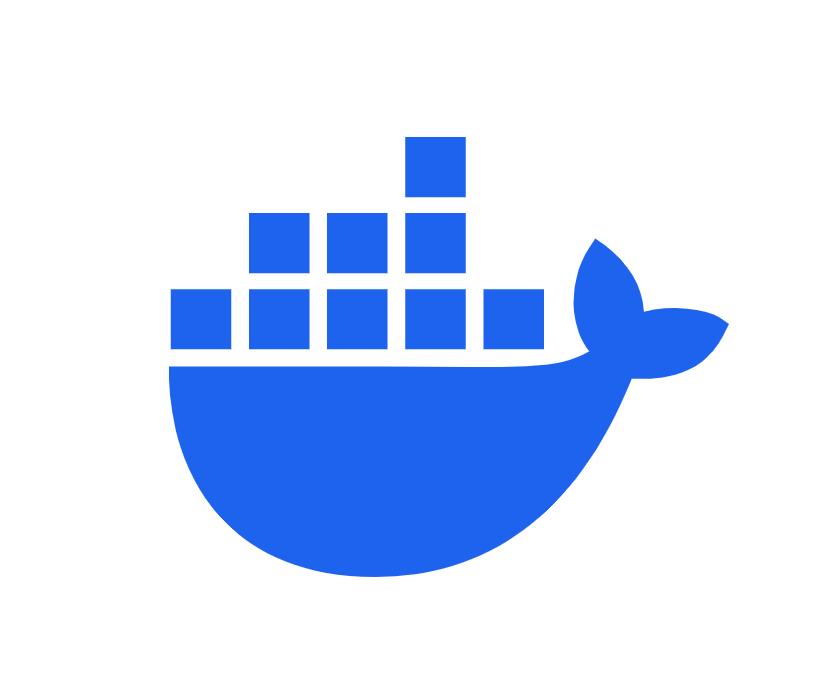
\includegraphics[width=0.2\linewidth]{figures/tech-logo/docker.png}
        \caption{Docker}
    \end{figure}
    \begin{itemize}
        \item \textbf{Khái niệm}: Docker là một nền tảng container hóa, cho
            phép đóng gói các ứng dụng và các phụ thuộc của chúng vào các
            container. Các container này có thể được chạy trên bất kỳ server nào
            có cài đặt Docker.

        \item \textbf{Ưu điểm}:
            \begin{itemize}
                \item Môi trường nhất quán: Đảm bảo rằng ứng dụng có thể hoạt
                    động trên bất kỳ môi trường.

                \item Mở rộng dễ dàng: Có thể dễ dàng mở rộng quy mô các ứng
                    dụng.

                \item Phân phối nhanh: Các container có thể được đóng gói và
                    phân phối một cách nhanh chóng.
            \end{itemize}

        \item \textbf{Ứng dụng trong dự án}: Tạo môi trường phát triển dưới local
            đơn giản và nhanh chóng, đóng gói các service vào các container
            riêng biệt. Từ đây có thể triển khai hệ thống lên môi trường sản phẩm
            cực kỳ dễ dàng.
    \end{itemize}

    % 2.10
    \section{Quản lý mã nguồn với Git/GitHub}
    \begin{figure}[H]
        \centering
        
\includegraphics[width=0.6\linewidth]{figures/tech-logo/git-github.png}
        \caption{Git \& GitHub}
    \end{figure}
    Git là một hệ thống quản lý phiên bản phân tán, cho phép theo dõi lịch sử
    thay đổi của mã nguồn. GitHub là một nền tảng dựa trên Git, cung cấp các
    tính năng cộng tác như fork, pull request, issue tracking.
\end{document}